\documentclass[12pt]{article}

\usepackage[margin=1in]{geometry}
\usepackage{hyperref}
\usepackage{amsmath}
\usepackage{graphicx}
\usepackage{float}


\title{Driving Tracker: User Document \\ CMPS 115 - Software Methodology}
\author{\\ \\ \\ Drifting Coders \\ \\ Ben D'Costa \\ Armando Silva \\ Vivian Tong \\ Danny Yeap \\ \\ \\}
\date{\today}

\begin{document}
\maketitle
\newpage

\tableofcontents
\newpage

\section{Overview}

The purpose of our project is to allow users to equalize the amount of driving amongst a group of friends, who frequently carpool together, so that one user is not burdened with driving duties. 

Driving Tracker is an Android application that aims to aid users in choosing a driver among a group of users by viewing how much each person has driven. The application records and updates the amount of ``driving" owed between the driver and passengers after the ride has ended. A user may also view the amount of ``driving" owed to friends.  

The application contains functionality for the user to create an account, create an event, view events, view log and add friends.

Our application is available for Android users.

\section{Documentation for User}

\subsection{Getting Started}
Follow these steps to get started with Driving Tracker: 
\begin{enumerate}
    \item Download the application from \url{https://github.com/dyeap/Carpool/blob/master/Driving_Tracker.apk}
    \item Install the application onto your Android device.
    \item Open the application on your device
        \begin{figure}[H]
            \centering
            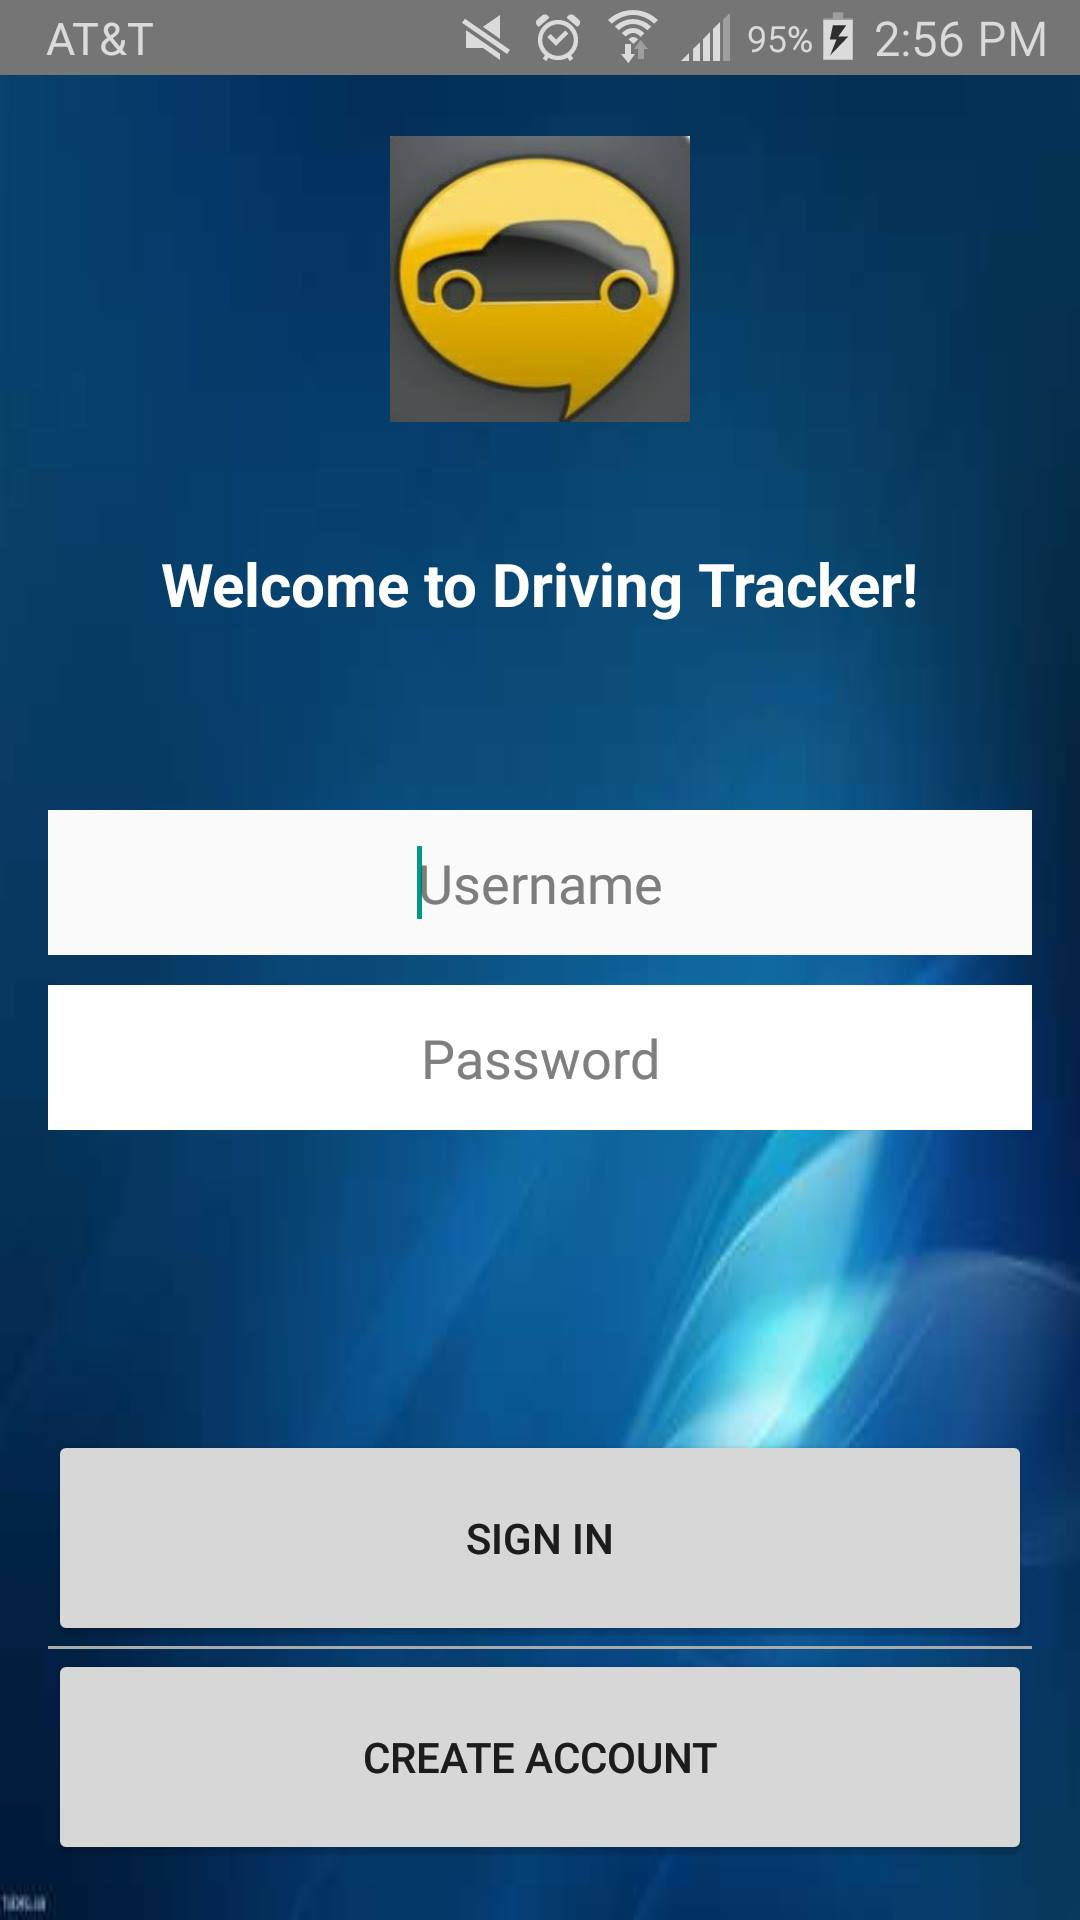
\includegraphics[width=1.5in]{log_in.jpg} 
            \caption{Start Page: Enter account information to sign in or create a new account.}
            \label{log_in}
        \end{figure}
    \item Create an account
        \begin{enumerate}
            \item Press "Create Account"
                \begin{figure}[H]
                    \centering
                    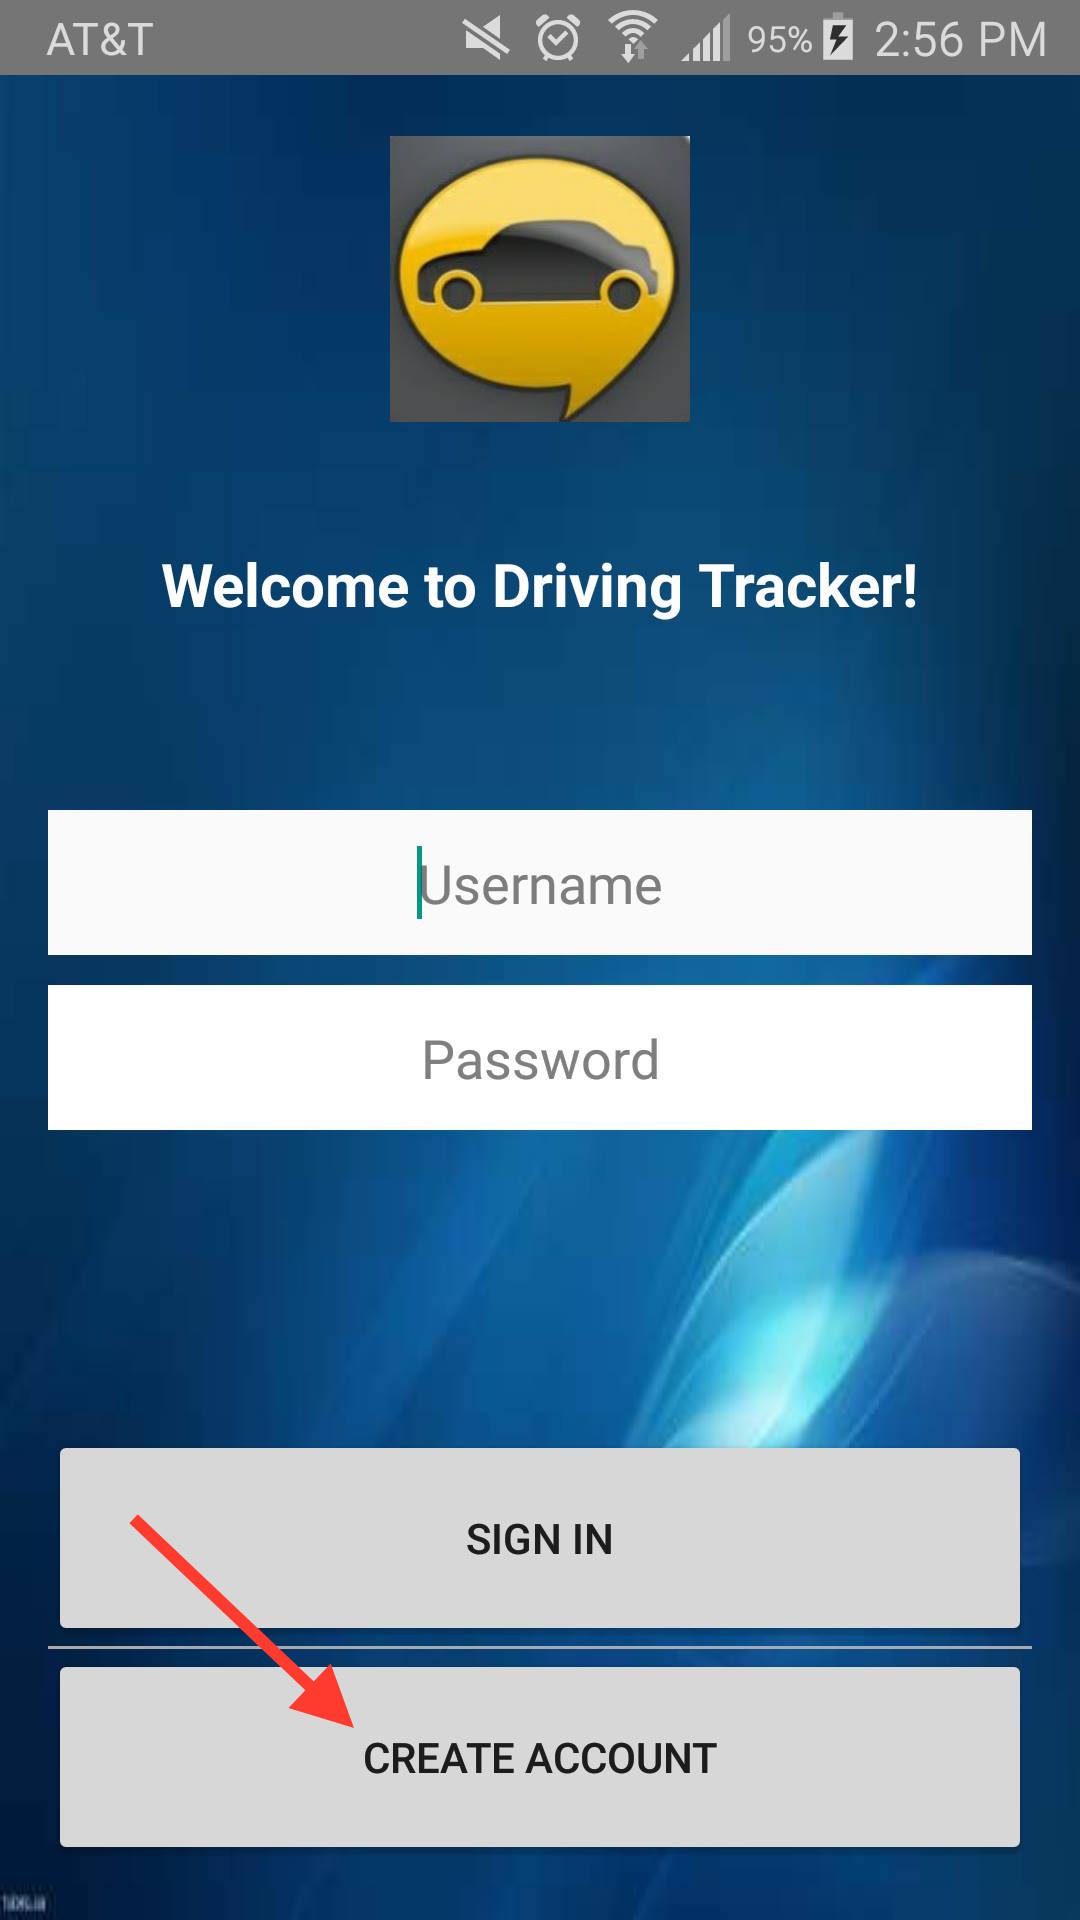
\includegraphics[width=1.5in]{log_in-create_acc.jpg}
                    \caption{Press ``Create Account,"  pointed by the red arrow, to begin creating a new account.}
                    \label{press_create_acc}
                \end{figure}
            \item{Enter username and password}
                \begin{figure}[H]
                    \centering
                    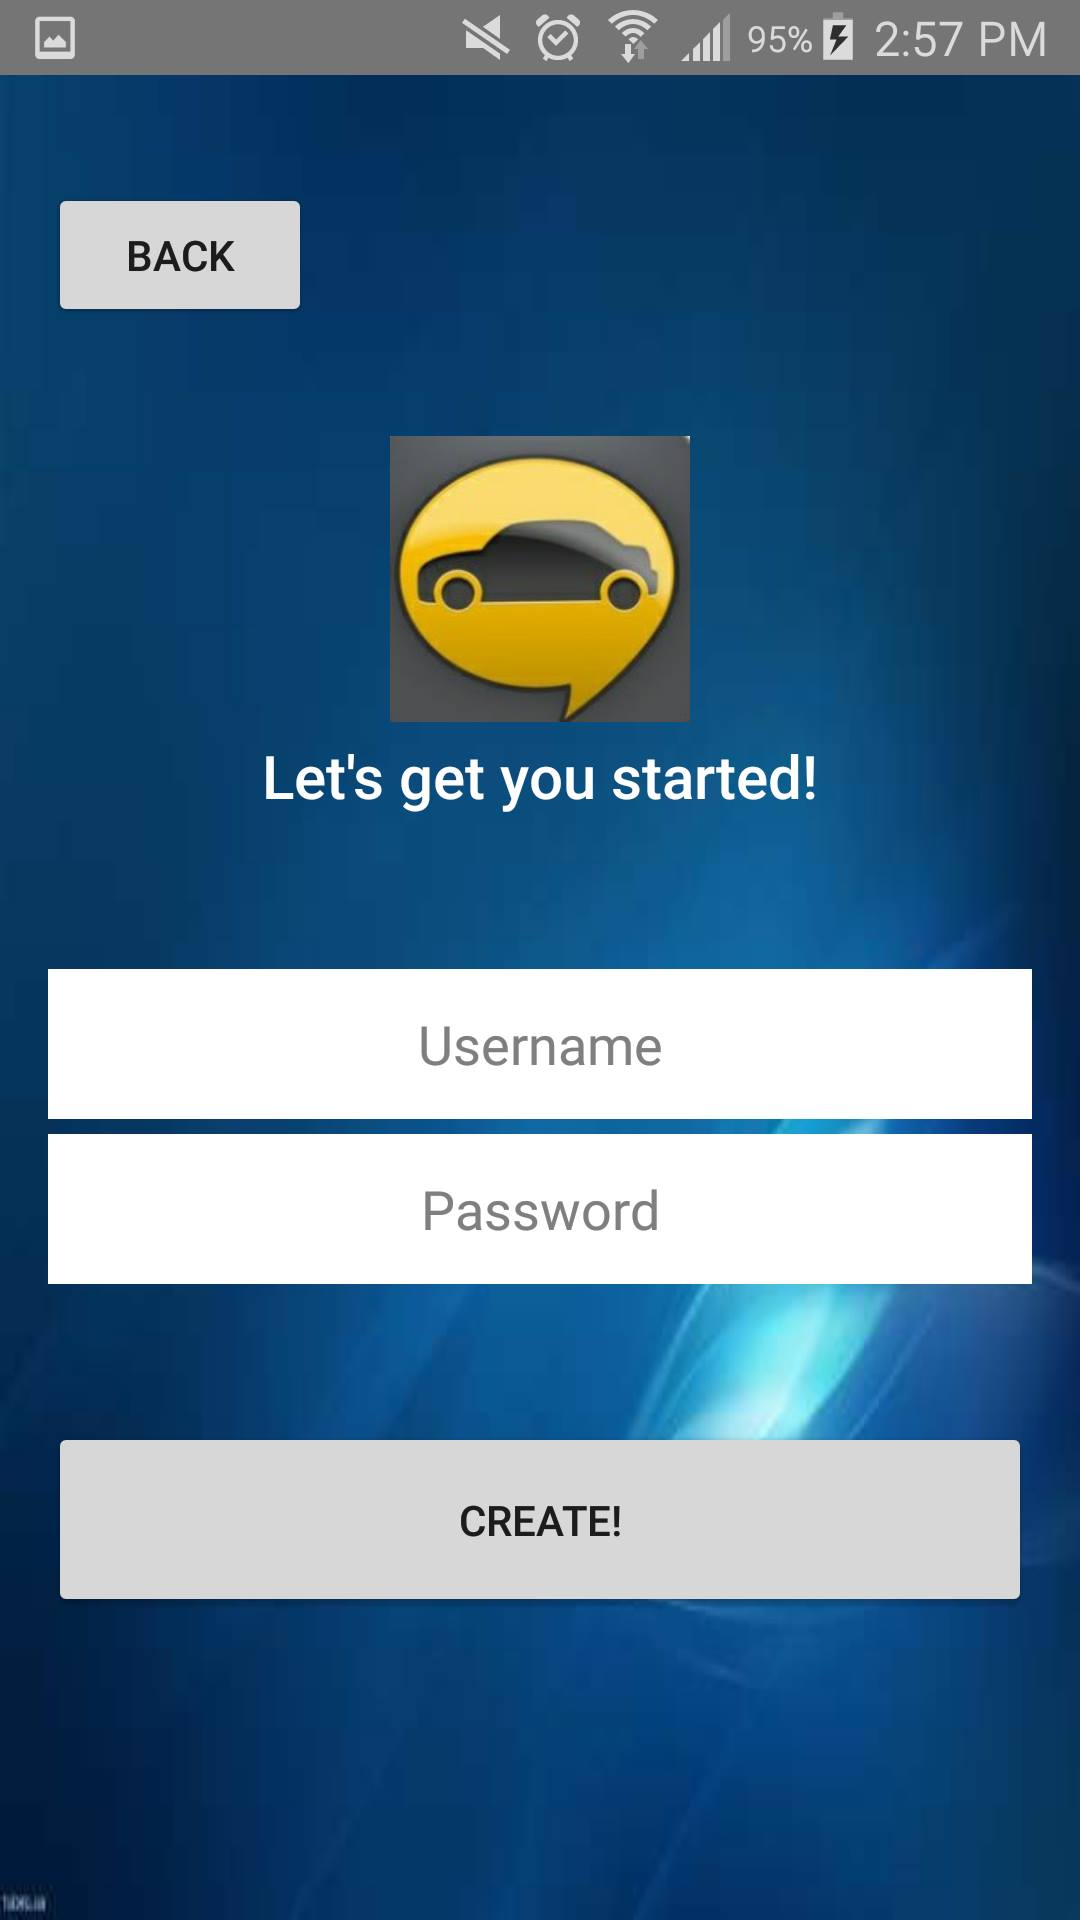
\includegraphics[width=1.5in]{create_acc.jpg}
                    \caption{Create Account Page: Enter desired username and password. Then, press ``Create!"}
                    \label{create_acc}
                \end{figure}
        \end{enumerate}
    \item Log in
        \begin{figure}[H]
            \centering
            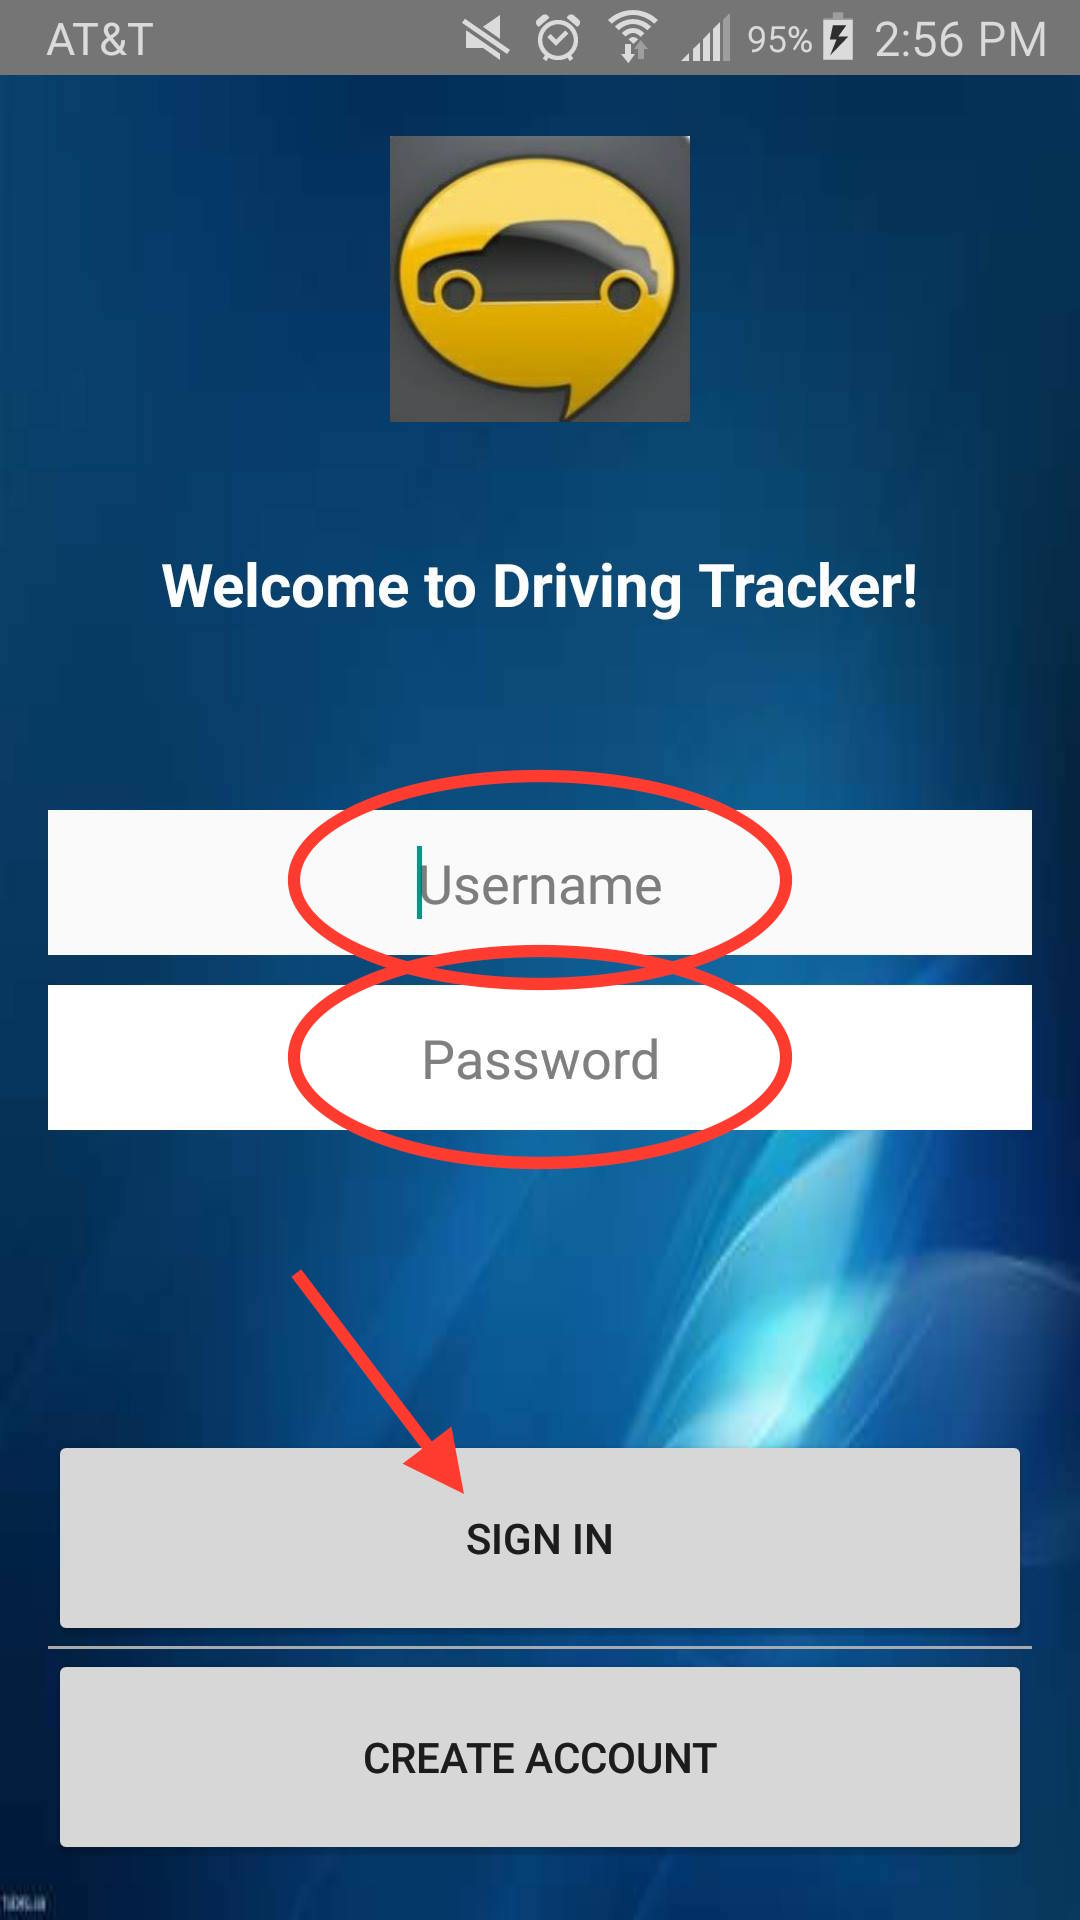
\includegraphics[width=1.5in]{logging_in.jpg}
            \caption{After pressing "Create!" from the previous page, you will be redirected to the start page.
            Log in by entering the username and password that was just created. Then, press ``Sign In."}
            \label{logging_in}
        \end{figure} 
        \begin{figure}[H]
            \centering
            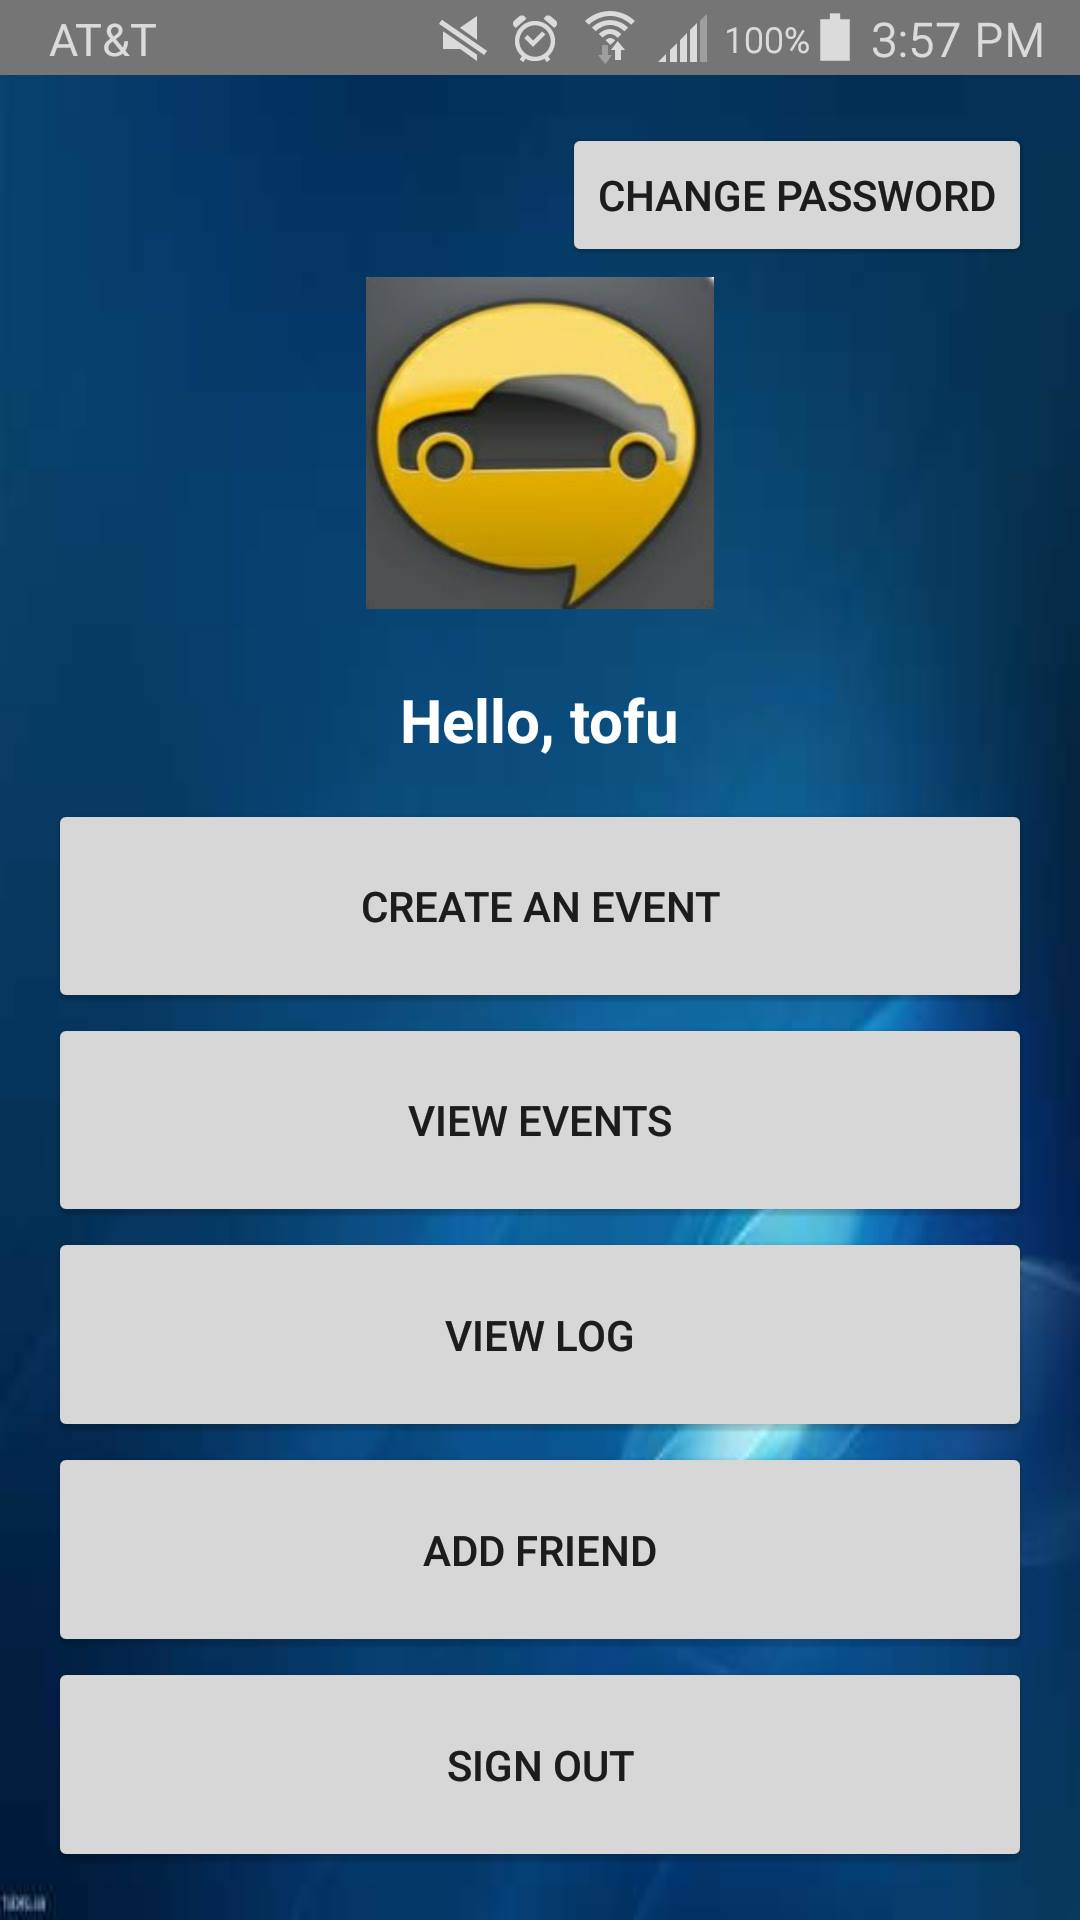
\includegraphics[width=1.5in]{account.jpg}
            \caption{After logging in, you will be redirected to your account page.}
            \label{account}
        \end{figure}
\end{enumerate}


\subsection{Application Features}
In the following examples,the username is tofu.
The following are the main features of the application:
\begin{itemize}
\item Create an Event
    \begin{figure}[H]
        \centering
        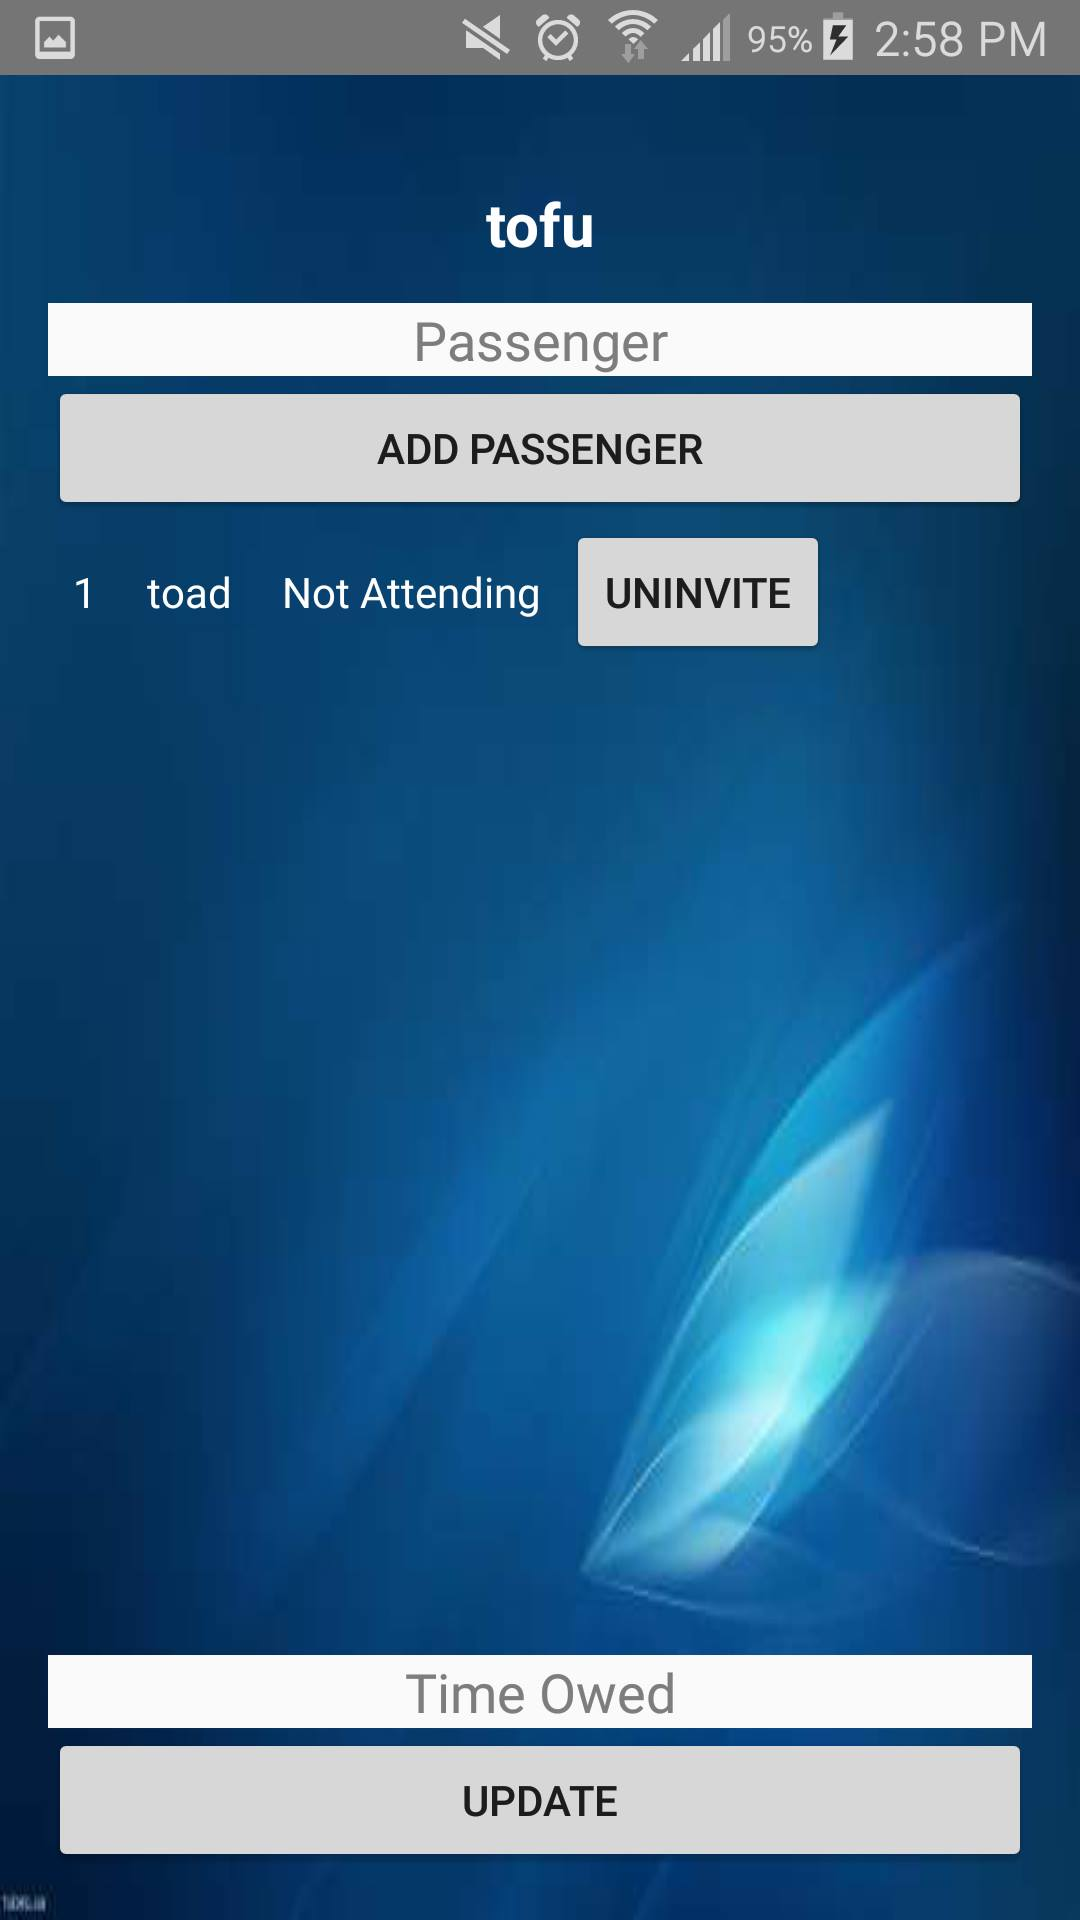
\includegraphics[width=1.5in]{create_event.jpg}
        \caption{Create Event Page: Add a friend as a passenger. The passenger may accept or decline.
        The user may also uninvited the invitee. At the end of the ride, the user can update the time owed, 
        which will update the log.}
        \label{create_event}
    \end{figure} 
\item View Events
    \begin{figure}[H]
        \centering
        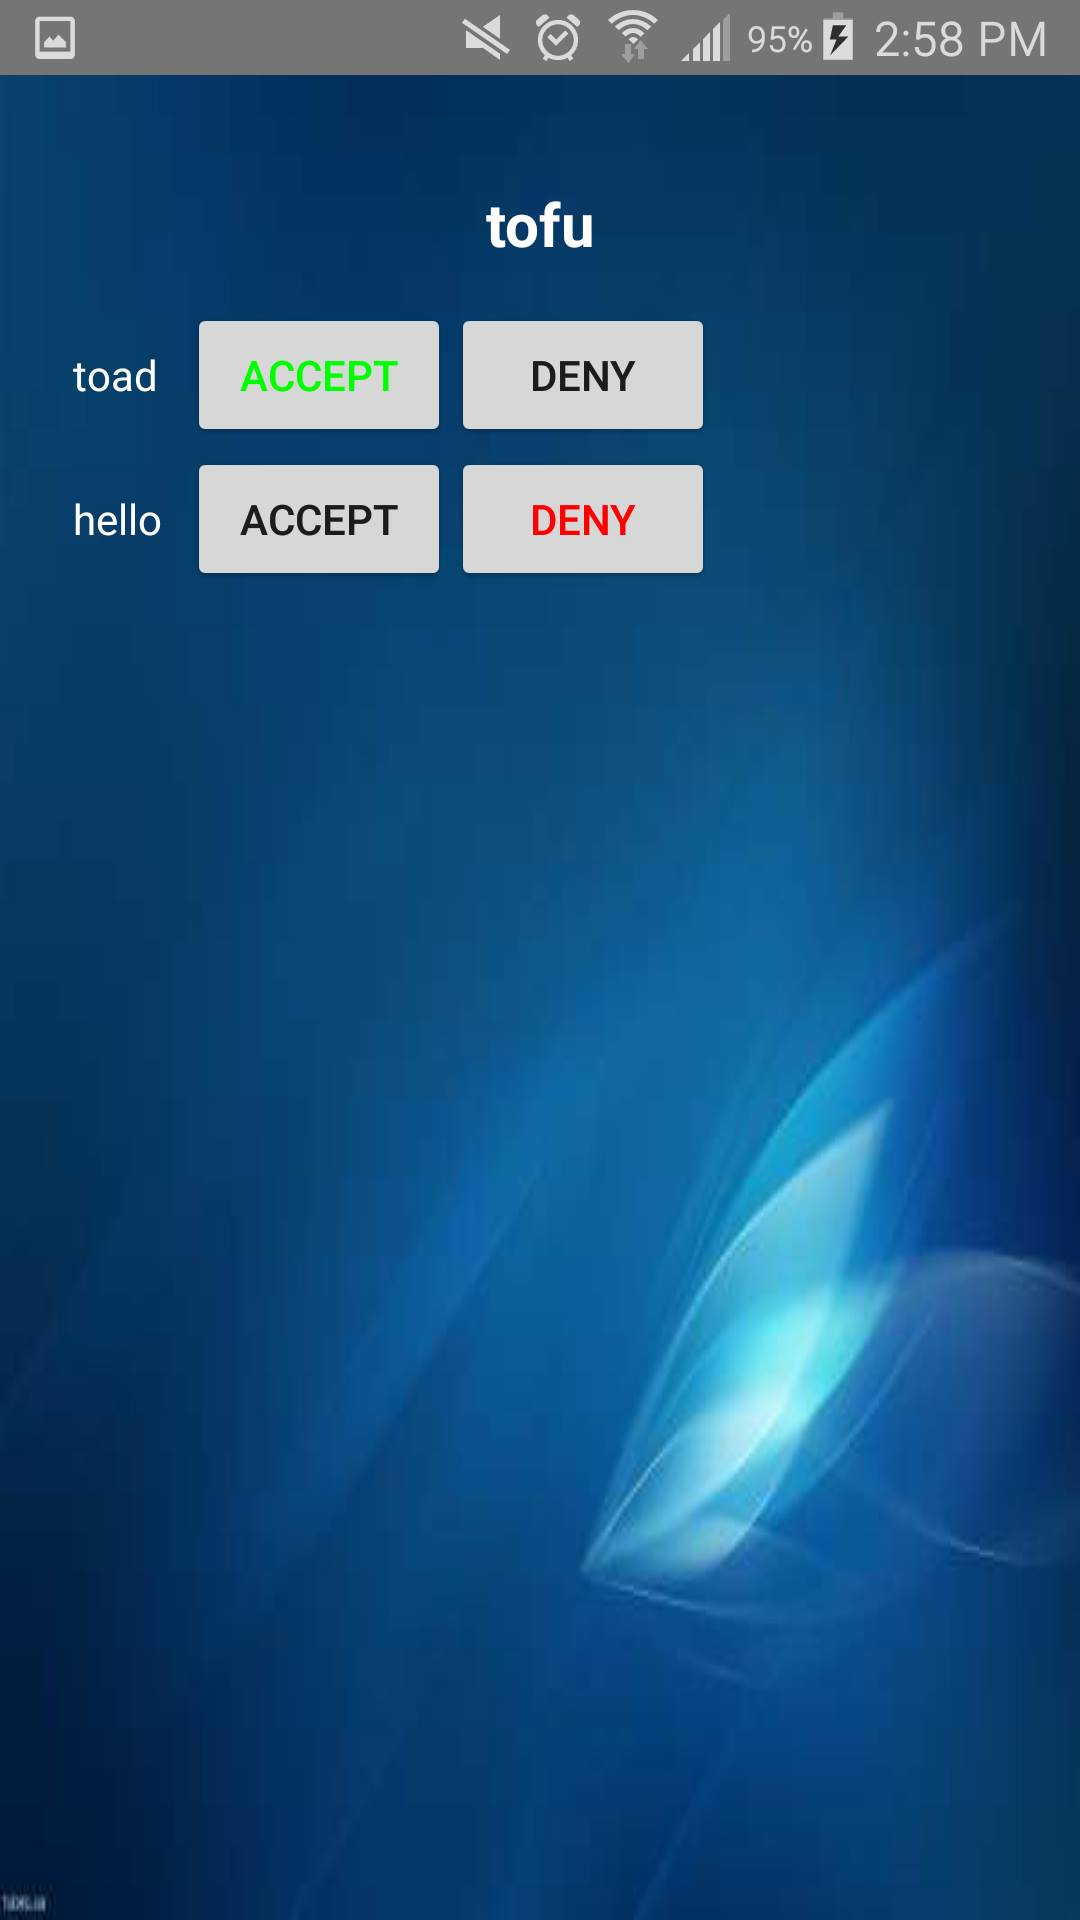
\includegraphics[width=1.5in]{view_events.jpg}
        \caption{View Events Page: The user has been invited to events by two friends. The user may accept 
        or decline the invitation. ``Accept" is highlighted by green, and ``Deny" is highlighted by red.}
        \label{view_events}
    \end{figure} 
\item View Log
    \begin{figure}[H]
        \centering
        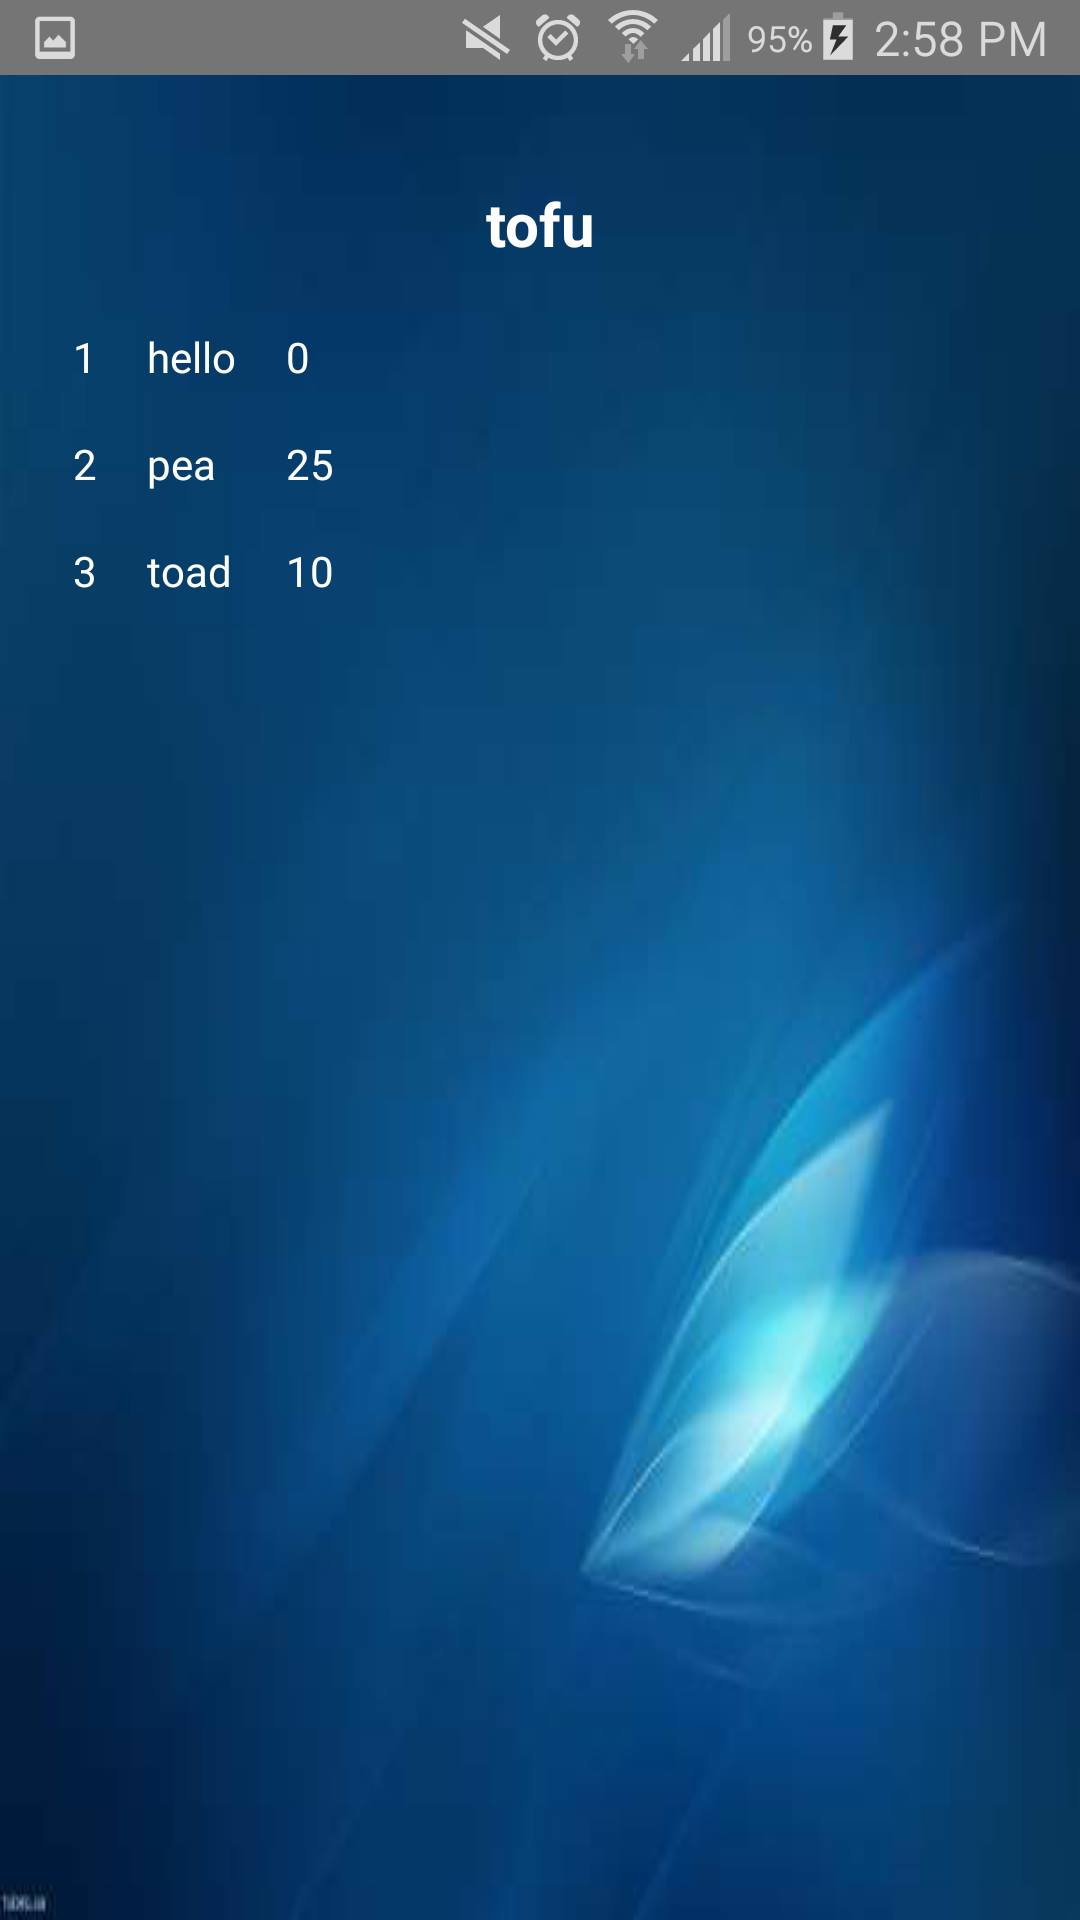
\includegraphics[width=1.5in]{view_log.jpg}
        \caption{View Log: Lists all the user's friends and how much they owe each other.}
        \label{view_log}
    \end{figure} 
\item Add Friend
    \begin{figure}[H]
        \centering
        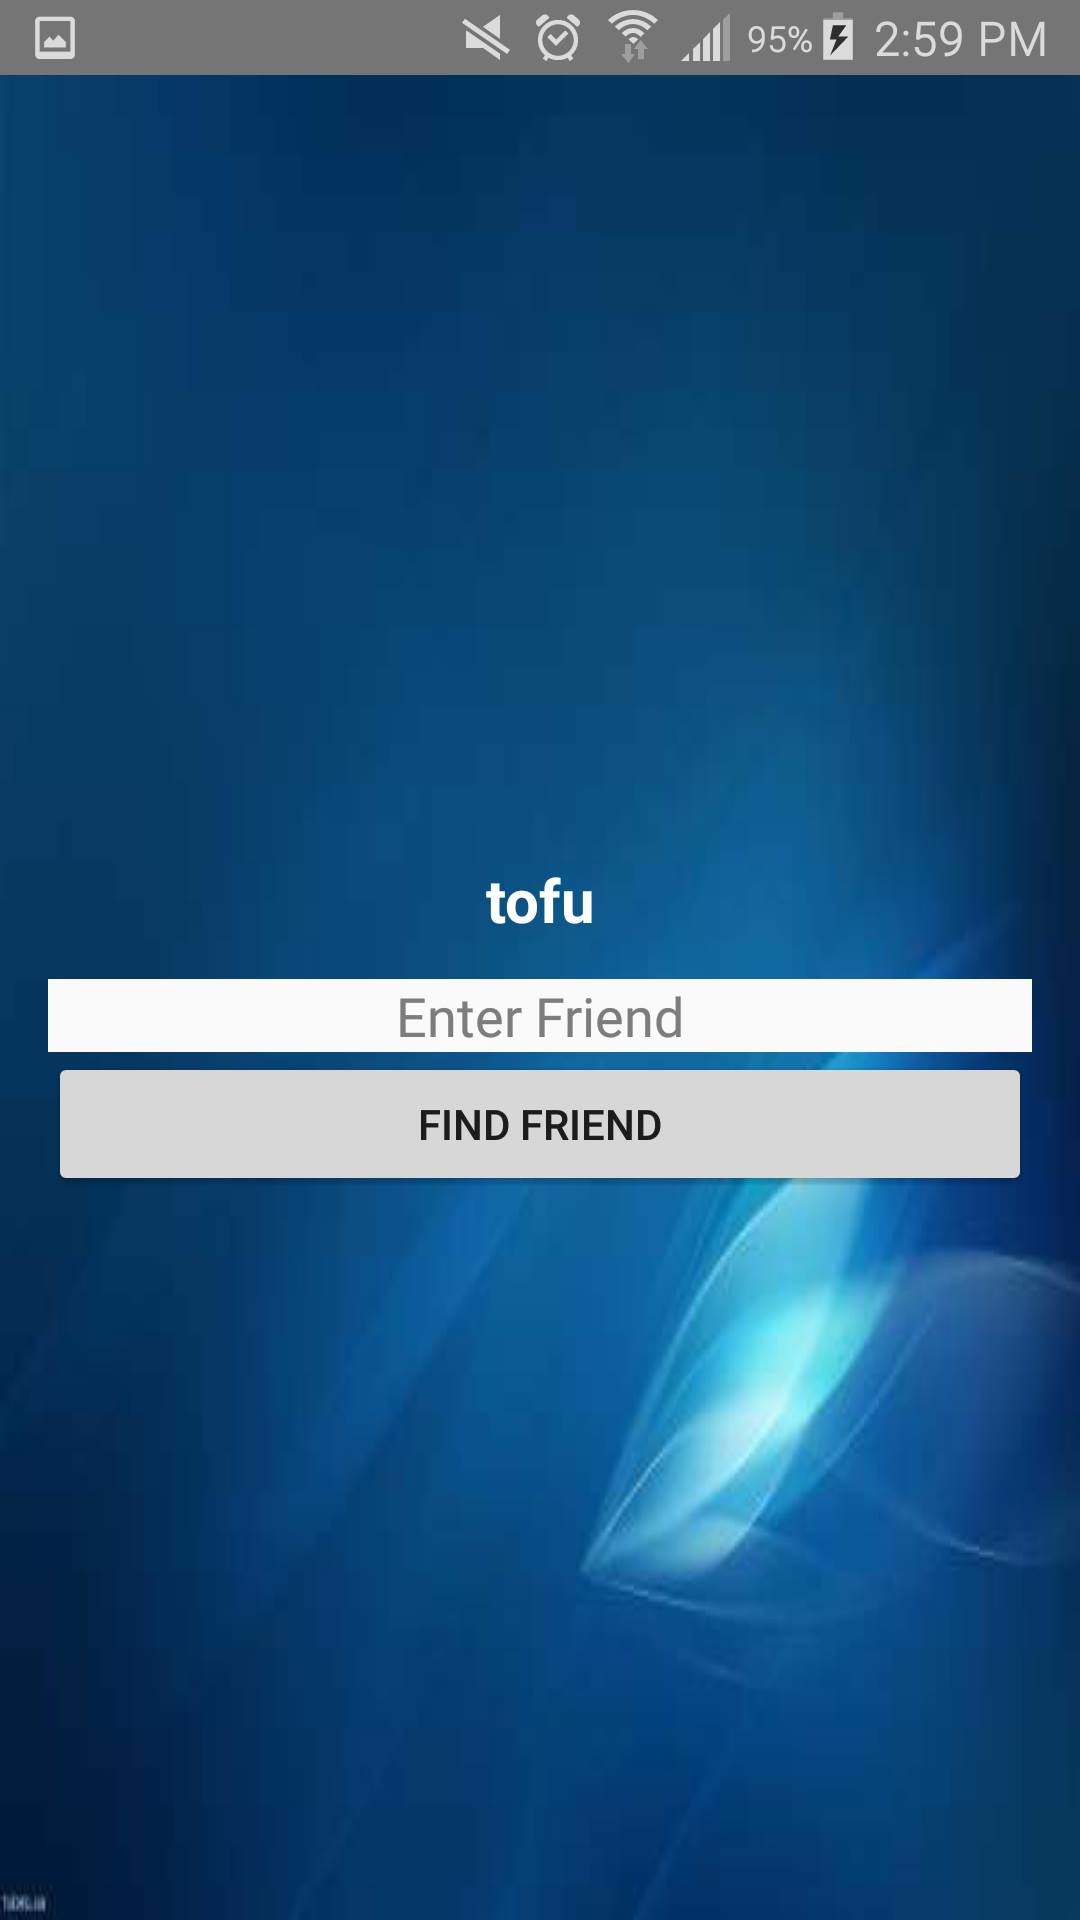
\includegraphics[width=1.5in]{add_friend.jpg}
        \caption{Add Friend: Before inviting friends to events or creating a log between the two users. One
        user must add the other user.}
        \label{add_friend}
    \end{figure} 
\end{itemize}



\section{Documentation for Developer}

\subsection{Setting Up the Environment}

\begin{enumerate}
\item Download the latest version of Android Studio at \url{http://developer.android.com/sdk/index.html}
\item Download the project from GitHub at \url{https://github.com/dyeap/Carpool}
\item Open the project in Android Studio

\begin{enumerate}
\item Click on the Android Studio application on your desktop
\item A ``Welcome to Android Studio" screen should appear. Select "Open an existing Android Studio project."
\item Select \textless Project Directory\textgreater /Sprint3/build.gradle
\end{enumerate}

\end{enumerate}

\subsection{Directory Structure}
Android Studio generates all the necessary files when a project is created. The files we, as developers, should focus on are activity files. Activity files are a subset of the source files that directly alter the application. An activity in an Android application is essentially a page of the application, so it is made up of a layout file (XML) that places the contents onto the page and a java file that controls the contents on the page. The activity files are organized by its type: XML or Java. Java files are located in $$ \text{\textless Project Directory\textgreater/Sprint3/ParseStarterProject/java/com.parse.starter} $$ Layout files are located in $$ \text{\textless Project Directory\textgreater/Sprint3/ParseStarterProject/res/layout/} $$ Another important file is strings.xml, which stores all the string variables for the layout files. It can be found at  $$ \text{\textless Project Directory\textgreater/Sprint3/ParseStarterProject/res/values/strings.xml} $$

\subsection{Parse}
We use Parse as our database. All user information is stored on Parse. Please contact the team for Parse
account information, if needed. User data could be found here:  
\begin{center}
\url{https://www.parse.com/apps/driving-tracker/collections}  
\end{center}
Useful resource for using Parse:  
\begin{center}
\url{https://parse.com/docs/android/guide#objects}
\end{center}
\end{document}

